\newpage
\section{Consuntivo di periodo}

In base ai consuntivi di periodo dei periodi completati sono state effettuate le diverse modifiche alla pianificazione per rientrare nel budget preventivato al momento della consegna per aggiudicarci il capitolato.
Di seguito sarà descritto il consuntivo di periodo di \PD\ e \COD\ da \RP\ fino alla \RQ.

\subsection{\PD\ e \COD\ da \RP\ fino alla \RQ}
La differenza di costi tra quelli preventivati nella sezione 5 di questo documento e quello effettivamente speso è la seguente:

\begin{table}[h]
	\begin{center}
		\begin{tabular}{|c|c|c|c|c|c|}
			\hline
			\textbf{Ruolo}	& \textbf{Ore Preventivate} & \textbf{Costo preventivato} &  \textbf{Differenza ore} & \textbf{Differenza costo} \\
			\hline
			\Pm &	11 & 330 & +2 & +60\\
			\hline
			\Am	&	6 & 120 & -1 & -20\\
			\hline
			\Prog	&	21 & 462 & +21 & +462\\
			\hline
			\Progr	&	193 & 2055 & +7 & +105\\
			\hline
			\Ver	&	91 & 1155 & +6 & +90\\
			\hline
			\textbf{totale}	&	\textbf{322} & \textbf{4122} & \textbf{+35} & \textbf{+697}\\
			\hline
		\end{tabular}
	\end{center}
	\caption{Consuntivo di periodo \PD\ e \COD\ da \RP\ fino alla \RQ}
\end{table}

\begin{figure}[H]
	\centering
	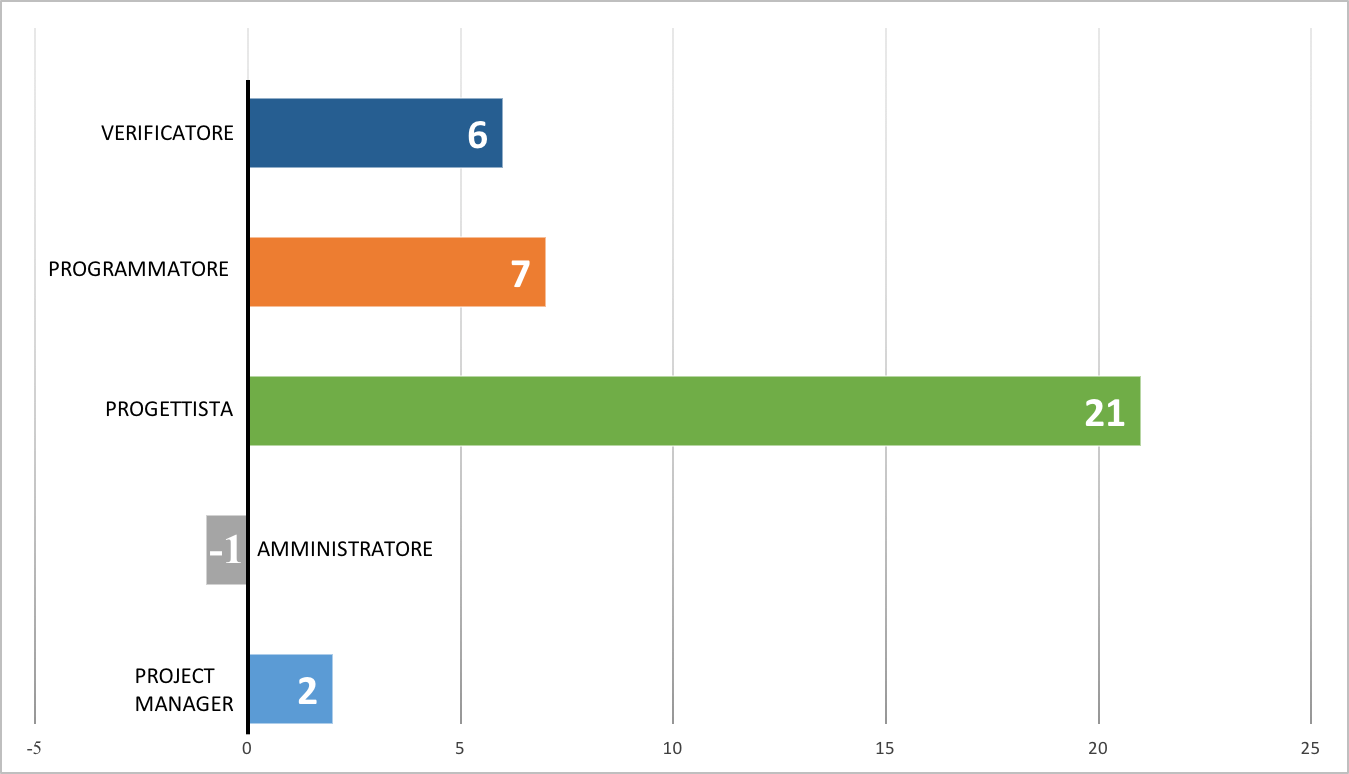
\includegraphics[scale=0.7]{Immagini/GraficiCONS/DIFFCONS.png}
	\caption{Differenza oraria per ruolo a consuntivo, Consuntivo di periodo \PD\ e \COD\ da \RP\ fino alla \RQ}
\end{figure}

Dal consuntivo di periodo emerge un aumento di \textbf{697\euro} nel preventivo a finire (che ora ammonta a \textbf{14318\euro}), rispetto ai \textbf{13621\euro} preventivati nella pianificazione ed al momento dell'aggiudicazione del capitolato.\\
Questo aumento è diretta conseguenza del verificarsi dei rischi descritti nella sezione 2 di questo documento.

Nonostante questo discostamento di 697\euro\ risultante dal consuntivo di periodo, il gruppo si impegna a rispettare l'impegno economico preso al momento dell'aggiudicazione del capitolato.\\
Infatti il gruppo è anche consapevole di aver superato le difficoltà di maggior peso e di aver già compiuto la maggior parte del lavoro richiesto per lo svolgimento del capitolato. Motivo per cui nell'ultimo periodo si prevede di rientrare nei costi preventivati di \textbf{13621\euro}. \\

\subsubsection{Preventivo a finire a seguito del consuntivo di periodo}
A seguito di una attenta analisi del consuntivo di periodo descritto appena sopra, la pianificazione dell'ultimo periodo rimanente (\VV) sarà modificata come segue:

\paragraph{Prospetto economico a seguito del consuntivo di periodo, \VV}
Nel periodo riguardante la \VV\ le ore tra i ruoli saranno divise nel seguente modo:
\begin{table}[h]
	\begin{center}
		\begin{tabular}{|l|c|c|}
			\hline
			\textbf{Ruolo}	& \textbf{Ore} &	\textbf{Costo}	 \\
			\hline
			\textit{\Pm}	&	8	&	240		\\
			\hline
			\textit{\Am}	&	3	&	60		\\ 
			\hline
			\textit{\Prog}	&	6	&	132	\\
			\hline
			\textit{\Progr}	&	8	&	120	\\ 
			\hline
			\textit{\Ver}	&	53	&	795	\\
			\hline
			\textbf{Totale}	&	\textbf{78}	&	\textbf{1347}	\\
			\hline
						
		\end{tabular}
	\end{center}
	\caption{Prospetto economico a seguito del consuntivo di periodo, \VV}
\end{table}

\begin{figure}[H]
	\centering
	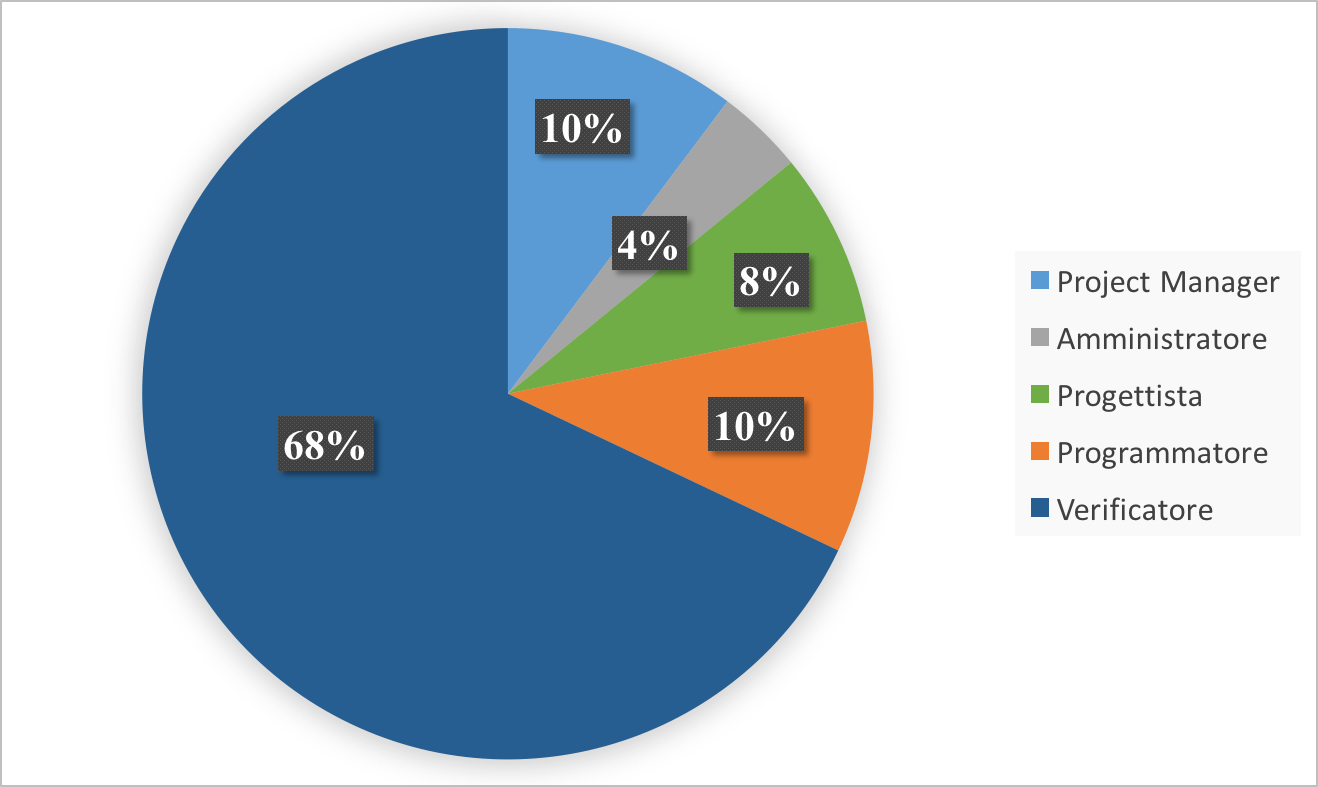
\includegraphics[scale=0.7]{Immagini/GraficiCONS/VVCONS.png}
	\caption{Incidenza ore per membro, \VV}
\end{figure}

\newpage
\paragraph{Prospetto economico a seguito del consuntivo di periodo, Totale}
A seguito di questa ri-pianificazione, le ore totali, previste per la realizzazione dell'intero progetto, comprese le ore di investimento e autoapprendimento, sono riportate nella tabella seguente:

\begin{table}[h]
	\begin{center}
		\begin{tabular}{|l|c|c|c|}
			\hline
			\textbf{Ruolo}	& \textbf{Ore} &	\textbf{Ore remunerabili}	 &\textbf{Costo} \\
			\hline
			\textit{\Pm}	&	57	&	37	&	1110	\\
			\hline
			\textit{\Am}	&	44	&	25	&	500	\\
			\hline
			\textit{\An}	&	105	&	30	&	750	\\
			\hline
			\textit{\Prog}	&	233	&	233	&	5126	\\
			\hline
			\textit{\Progr}	&	208	&	152	&	2280	\\
			\hline
			\textit{\Ver}	&	306	&	257	&	3855	\\
			\hline
			\textbf{Totale}	&	\textbf{953} & \textbf{734} & \textbf{13621}	\\
			\hline
		\end{tabular}
	\end{center}
	\caption{Costo totale per ruolo in seguito a ripianificazione}
\end{table}

\begin{figure}[H]
	\centering
	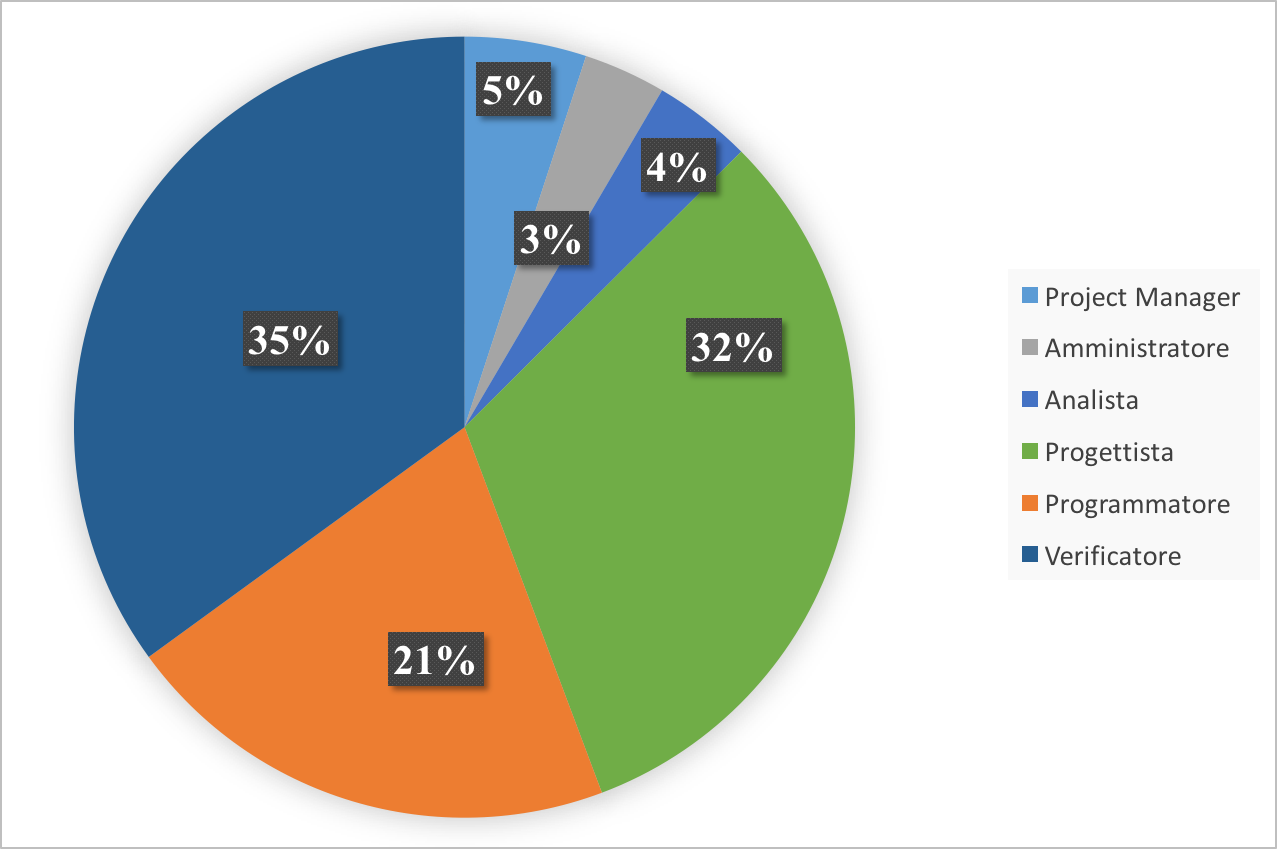
\includegraphics[scale=0.7]{Immagini/GraficiCONS/TOTCONS.png}
	\caption{Prospetto economico a seguito del consuntivo di periodo, Totale}
\end{figure}

Il gruppo quindi, seguendo questa ri-pianificazione per l'ultimo periodo rimanente, riesce a rientrare e a rispettare il preventivo di \textbf{13621\euro} fissato al momento dell'aggiudicazione del capitolato.